\documentclass[11pt]{article}
\usepackage[T1]{fontenc}
\usepackage[utf8]{inputenc}
\usepackage{lmodern}
\usepackage[margin=1.15in]{geometry}
\usepackage{amsmath,amssymb,amsthm,mathtools}
\usepackage{microtype}
\usepackage{booktabs}
\usepackage{pgfplots}
\pgfplotsset{compat=1.16}
\usepackage[hidelinks]{hyperref}
\usepackage{setspace}
\setstretch{1.08}

\newtheorem{theorem}{Theorem}[section]
\newtheorem{proposition}[theorem]{Proposition}
\newtheorem{corollary}[theorem]{Corollary}
\theoremstyle{definition}
\newtheorem{definition}[theorem]{Definition}
\newtheorem{assumption}[theorem]{Assumption}
\theoremstyle{remark}
\newtheorem{remark}[theorem]{Remark}
\newtheorem{nonsupport}{Statement of Non-Support}

\newcommand{\E}{\mathbb{E}}
\newcommand{\Prob}{\mathbb{P}}
\newcommand{\R}{\mathbb{R}}
\newcommand{\ind}{\mathbf{1}}
\newcommand{\MI}{\mathsf{MI}}
\newcommand{\Ent}{\mathsf{H}}

\title{The Perpetual Renovation Theorem\\[0.5em]
\large Urban Saturation, Gratuitous Replacement, and the Acoustic Commons}
\author{Flyxion\\ Independent Researcher}
\date{October 2026}

\begin{document}
\maketitle

\begin{abstract}
\noindent A minor genre of informal video commentary has grown up around life in very large and very dense cities, and one of its recurring complaints is the near-continuous percussive noise of demolition work, attributed by speakers to renovation in which intact floor tile is broken out with electric breakers and replaced with new tile. This paper constructs a family of stylized stochastic and game-theoretic models in which such a condition can arise, and proves seven results about them. A decoupling theorem shows that when the decision to replace a building component depends on private ledger variables and not on its physical condition, the replaced stock is a representative sample of the whole stock, so that adequate components are destroyed at exactly the rate at which they exist (the Functional Adequacy Paradox). An exact silence law shows that the probability that a resident hears no renovation decays geometrically in the number of audible units even when each unit's own duty cycle is small, and that statutory quiet hours become the only quiet that survives at scale (the Acoustic Commons Theorem). A mean-free-path law gives the average acoustic intensity supplied by a Poisson field of active sources, with the many setting the mean and the nearest setting the fluctuation (the Renovation Olbers Theorem). A collapse result shows that marginal-harm pricing of noise tends to zero as the audience saturates. Finally, a symmetric renovation game exhibits a regime in which measured output rises while welfare falls below zero (the Perpetual Reconstruction Equilibrium). Two further results are drawn from the literary Shangri-La, where the audible set is empty: a bounded-harm result showing that the resident of a sufficiently large city rationally declines the silent valley (Conway's Dilemma), and a fixed-point result showing that advertising a silent place lowers its silence monotonically (the Shangri-La Paradox). Every theorem is conditional on its hypotheses, and the hypotheses are stated. None of these results supports or proves the motivating hypothesis that any particular share of real renovation is unnecessary, that any particular city exhibits the equilibrium described, or that the complaint genre is representative of anything. The paper does not support its own hypothesis, and repeats this in each section.
\end{abstract}

\section{Introduction}

A minor genre of informal video commentary has accumulated around the experience of living in very large and very dense cities. Among its recurring complaints, in recordings made by residents and visitors in Tokyo and in several Chinese metropolitan regions, is the persistence of percussive demolition noise through the working day. The speakers commonly attribute it to renovation that includes the removal of floor tile by electric breakers and its replacement by new tile, in circumstances where the removed tile is described as having been in serviceable condition, and more generally to a continual cycle of construction and reconstruction that never appears to rest. The genre is anecdotal, self-selected and unsystematic. It is treated here as a source of questions and not as a source of evidence.

The complaint has a precise formal core. Maintenance is a response to physical decline: a component is replaced when its functional quality falls below a technical threshold. Renovation is a response to a ledger: a component is replaced when the sum of the gain, incentive and prestige attached to replacement exceeds its cost to the party who decides. The two decision rules coincide only if the ledger tracks physical condition, and there is no general reason why it should. A tiled floor in good repair may represent an absence of demand to its occupant, a stream of revenue to its contractor, an asset improvement to its owner and a demonstration of activity to its manager, so that the same object occupies incompatible positions in several accounting systems. Its physical adequacy then fails to protect it from replacement. The remaining question is what happens when thousands of such decisions, each individually permissible and each individually modest, are made independently within earshot of one another.

The contributions of the paper are seven formal results, each stated with hypotheses and proved. Section~\ref{sec:setting} fixes notation. Section~\ref{sec:adequacy} proves the decoupling theorem and a companion result on an obsolescence chain. Section~\ref{sec:commons} proves the exact silence law and a corollary on mandated quiet. Section~\ref{sec:olbers} proves the mean-free-path law. Section~\ref{sec:collapse} proves the collapse of marginal-harm pricing. Section~\ref{sec:equilibrium} defines and characterizes the Perpetual Reconstruction Equilibrium. Section~\ref{sec:shangri} treats the Shangri-La limit of the empty audible set. Section~\ref{sec:discussion} states what the models omit, including the best counterexample to the motivating hypothesis that the author was able to find, and Section~\ref{sec:conclusion} concludes.

The paper draws on several literatures without contributing to any of them. The theory of externalities begins with Pigou~\cite{pigou} and is complicated by Coase~\cite{coase}. The commons problem is classically stated by Hardin~\cite{hardin} and qualified by Ostrom~\cite{ostrom}, and the logic of dispersed beneficiaries and concentrated costs follows Olson~\cite{olson}. The idea that destruction can be productive appears in Schumpeter~\cite{schumpeter} and in its sharpest rebuttal in Bastiat~\cite{bastiat}, whose broken window is the intellectual ancestor of the broken tile. Prestige-driven consumption is Veblen's subject~\cite{veblen}, divergence between an actor's interest and the interest of those who bear the consequences is the subject of agency theory~\cite{jensen}, and the layering of building components by rate of change is described by Brand~\cite{brand}. On the stochastic side the paper uses superposition of renewal processes~\cite{cox,khinchin}, Poisson point processes and Campbell's theorem~\cite{campbell,kingman}, and a classical argument from observational cosmology~\cite{harrison}. The limiting case of an empty audible set is supplied by Hilton's \emph{Lost Horizon}~\cite{hilton}.

\begin{nonsupport}\label{ns:intro}
The hypothesis that motivates this paper is the following. \emph{H: a non-negligible share of the demolition noise in dense metropolitan housing is produced by replacement of components that are physically adequate.} This paper does not support H. No data are analyzed. The models below are consistent with H, and they are equally consistent with its negation, because the parameter that would separate the two, the gratuitous fraction of replacements, is left free throughout. A reader who finishes the paper believing H has been persuaded by something other than the paper.
\end{nonsupport}

\section{Setting and Notation}\label{sec:setting}

Fix a reference resident. The \emph{audible set} is the finite collection of $n$ dwelling units whose renovation work the resident can hear, whether through air, through structure, or through both. Each unit contains components indexed by $k$, of which the canonical example is a tiled floor. Let $N$ be the number of occupants of a metropolitan region and $A$ its usable floor area, and define the saturation $\sigma = N/A$. The size of the audible set is assumed to depend on saturation in the following weak sense.

\begin{assumption}[Saturation scaling]\label{as:scaling}
The audible set size $n = n(\sigma)$ is nondecreasing and unbounded in $\sigma$.
\end{assumption}

For a component $k$, let $Q_k(t)\in[0,1]$ denote its functional quality at time $t$, and let $\theta_k$ be the threshold below which replacement is technically justified. The \emph{technical replacement time} is $\tau_k = \inf\{t : Q_k(t) < \theta_k\}$. Ordinary maintenance replaces a component at $\tau_k$, which is the same as the rule $R^{\mathrm{M}}_k(t) = \ind[Q_k(t) < \theta_k]$.

Let the \emph{ledger vector} of the deciding party be $V_k(t) = (G_k, I_k, \Pi_k, C_k)(t)$, where $G_k$ is anticipated financial gain, $I_k$ is the institutional incentive attached to replacement, $\Pi_k$ is perceived prestige or aesthetic improvement, and $C_k$ is the cost of renovation to the decider. The ledger rule replaces a component when
\begin{equation}\label{eq:ledger}
R_k(t) = \ind\bigl[\,G_k(t) + I_k(t) + \Pi_k(t) > C_k(t)\,\bigr].
\end{equation}
Four quantities are absent from \eqref{eq:ledger}: the acoustic burden on occupants of the audible set, the disruption of neighboring activity, the embodied material utility destroyed by the replacement, and the opportunity cost of the labor diverted to it. Call their sum the \emph{external bundle} $E_k$. A replacement is \emph{gratuitous} if it occurs while the component is physically adequate, that is, on the event $\{R_k = 1\}\cap\{Q_k \ge \theta_k\}$. Table~\ref{tab:notation} collects the symbols used in later sections.

\begin{table}[ht]
\centering
\small
\begin{tabular}{@{}cp{5.2cm}@{\hspace{1em}}cp{5.2cm}@{}}
\toprule
Symbol & Meaning & Symbol & Meaning \\
\midrule
$n$ & size of the audible set & $\mu$ & physical failure rate of a component \\
$\epsilon$ & duty cycle of a unit & $\omega$ & rate at which a component becomes obsolete \\
$\lambda$ & renovation rate per unit & $r$ & rate at which obsolescence is acted upon \\
$d$ & mean duration of an episode & $\nu$ & spatial density of active sources \\
$\rho$ & expected active sources, $n\epsilon$ & $\kappa$ & absorption coefficient \\
$\varphi$ & fraction of time in which work is permitted & $h$ & harm per unit renovation rate to one other unit \\
$a,b,c$ & benefit and cost parameters & $\eta$ & external burden, $(n-1)h$ \\
$B,v$ & agglomeration benefit, harm value & $m,n_0$ & attraction parameter, baseline audible set \\
\bottomrule
\end{tabular}
\caption{Notation used in Sections~\ref{sec:adequacy} through~\ref{sec:shangri}.}\label{tab:notation}
\end{table}

\section{The Functional Adequacy Paradox}\label{sec:adequacy}

The first result formalizes the observation that a decision rule built from ledger variables carries no information about physical condition unless the ledger is coupled to condition by some mechanism.

\begin{definition}[Functional Adequacy Paradox]
A replacement regime exhibits the Functional Adequacy Paradox when the probability that a replaced component is physically adequate is positive, and in the limiting case equals the probability that an arbitrary component of the stock is physically adequate.
\end{definition}

\begin{theorem}[Decoupling]\label{thm:decoupling}
Let $(Q, V)$ be the quality and ledger vector of a component at a decision time, and let $R = f(V)$ be any measurable decision rule, in particular \eqref{eq:ledger}. If $V$ is independent of $Q$, then
\begin{enumerate}
\item[(a)] the mutual information $\MI(R;Q)$ is zero;
\item[(b)] for every threshold $\theta$ and whenever $\Prob(R=1)>0$, $\Prob(Q\ge\theta \mid R=1) = \Prob(Q\ge\theta)$;
\item[(c)] in a stock of $m$ independent and identically distributed components, the expected number of gratuitous replacements is $m\,\Prob(R=1)\,\Prob(Q\ge\theta)$.
\end{enumerate}
By contrast, under maintenance $R^{\mathrm{M}} = \ind[Q<\theta]$ one has $\MI(R^{\mathrm{M}};Q) = \Ent(R^{\mathrm{M}})$, the binary entropy of the replacement event, and no replacement is gratuitous.
\end{theorem}

\begin{proof}
The random variable $R$ is a measurable function of $V$, so the $\sigma$-algebra it generates is contained in that of $V$ and is therefore independent of that generated by $Q$. Independent random variables have zero mutual information~\cite{cover}, which gives (a). For (b), independence gives $\Prob(Q\ge\theta, R=1) = \Prob(Q\ge\theta)\Prob(R=1)$, and dividing by $\Prob(R=1)$ yields the claim. For (c), linearity of expectation over the $m$ components applied to the indicator of $\{R=1\}\cap\{Q\ge\theta\}$ gives $m\Prob(R=1,Q\ge\theta)$, which factors by independence. For the contrast, $R^{\mathrm{M}}$ is a deterministic function of $Q$, so $\MI(R^{\mathrm{M}};Q) = \Ent(R^{\mathrm{M}}) - \Ent(R^{\mathrm{M}}\mid Q) = \Ent(R^{\mathrm{M}})$, and on $\{R^{\mathrm{M}}=1\}$ one has $Q<\theta$ by construction.
\end{proof}

The theorem has an uncomfortable reading. If the ledger is independent of condition, then the floors that are broken out are a fair sample of all floors, and the proportion of broken-out floors that were adequate equals the proportion of floors that were adequate. A regime in which most floors are adequate is a regime in which most destroyed floors were adequate. Independence is an extreme case, and the realistic case is partial coupling in which condition enters $V$ weakly, but the extreme case identifies the quantity that matters, namely how strongly condition enters the ledger.

A second, dynamic route to the same conclusion does not require independence of any state variable. Suppose that a component, once installed, passes through three conditions. It begins \emph{current}, becomes \emph{obsolete but functional} at rate $\omega$ as fashion, regulation or resale expectation moves on, and in either condition fails physically at rate $\mu$. An obsolete component is replaced by choice at rate $r$, which measures how readily the deciding party acts on obsolescence. Any failure or replacement returns the cycle to the current condition. All sojourns are independent and exponential.

\begin{proposition}[Obsolescence Chain]\label{prop:chain}
In the chain above, (i) the long-run replacement rate per component is
\begin{equation}\label{eq:rate}
\lambda(\mu) = \frac{(\omega+\mu)(r+\mu)}{\omega+r+\mu},
\end{equation}
and (ii) the fraction of replacements that are gratuitous is
\begin{equation}\label{eq:pg}
p_G = \frac{\omega}{\omega+\mu}\cdot\frac{r}{r+\mu}.
\end{equation}
\end{proposition}

\begin{proof}
A cycle begins in the current condition, whose exit rate is $\omega+\mu$ and whose mean sojourn is $1/(\omega+\mu)$. With probability $\omega/(\omega+\mu)$ the exit is to obsolescence, where the exit rate is $r+\mu$ and the mean sojourn is $1/(r+\mu)$. The mean cycle length is therefore
\[
\E[T] = \frac{1}{\omega+\mu} + \frac{\omega}{\omega+\mu}\cdot\frac{1}{r+\mu} = \frac{\omega+r+\mu}{(\omega+\mu)(r+\mu)},
\]
and the renewal rate $\lambda = 1/\E[T]$ is \eqref{eq:rate}. A cycle ends in a gratuitous replacement exactly when the first exit is to obsolescence and the second exit is by choice, an event of probability $\frac{\omega}{\omega+\mu}\cdot\frac{r}{r+\mu}$. Each cycle contains one replacement, so this is also the gratuitous fraction among replacements.
\end{proof}

\begin{corollary}[First-Order Insensitivity to Decay]\label{cor:insens}
To first order in $\mu$,
\[
\lambda(\mu) = \frac{\omega r}{\omega+r} + \mu\Bigl[1 - \frac{\omega r}{(\omega+r)^2}\Bigr] + O(\mu^2),
\]
so the elasticity of the replacement rate with respect to the physical failure rate is bounded, to first order, by $\mu\,(1/\omega + 1/r)$. In the limit $\mu\to0$, the replacement rate satisfies $1/\lambda = 1/\omega + 1/r$ and does not depend on $\mu$ at all, and $p_G\to1$.
\end{corollary}

\begin{proof}
Differentiate \eqref{eq:rate} at $\mu=0$: with $N(\mu)=\omega r+(\omega+r)\mu+\mu^2$ and $D(\mu)=\omega+r+\mu$, one has $\lambda'(0) = [(\omega+r)^2-\omega r]/(\omega+r)^2$. The elasticity $\mu\lambda'/\lambda$ is then $\mu\,\frac{\omega+r}{\omega r}\bigl[1-\frac{\omega r}{(\omega+r)^2}\bigr]$ to first order, and $\frac{\omega+r}{\omega r} = \frac1\omega+\frac1r$. The limits follow by setting $\mu=0$ in \eqref{eq:rate} and \eqref{eq:pg}.
\end{proof}

The corollary can be read as a statement about what the replacement rate measures. Under maintenance ($\omega=0$) one recovers $\lambda=\mu$, so the rate of replacement is the rate of decay. Under a regime in which obsolescence and readiness are fast relative to decay, the rate of replacement is the series combination of two clocks, neither of which is physical, and the building is renewed on a schedule set by fashion and by the speed of the deciding party.

\begin{nonsupport}\label{ns:adequacy}
Theorem~\ref{thm:decoupling} and Proposition~\ref{prop:chain} do not support H. They show what would follow if the ledger were independent of condition, or if $\omega$ and $r$ were large relative to $\mu$. The paper does not estimate $\omega$, $r$ or $\mu$ for any building, city or country, and it does not prove that the independence hypothesis holds anywhere. The result is a conditional implication whose antecedent is not established.
\end{nonsupport}

\section{The Acoustic Commons Theorem}\label{sec:commons}

Consider the audible set of Section~\ref{sec:setting}. Each unit alternates between idle periods and active renovation periods, forming an alternating renewal process. Let $\lambda$ be the long-run rate of renovation cycles per unit time and $d$ the mean duration of an active period, so that the stationary \emph{duty cycle}, the long-run fraction of time the unit is active, is $\epsilon = \lambda d$, with $0<\epsilon<1$.

\begin{assumption}[Independence and homogeneity]\label{as:indep}
The $n$ units are stochastically identical with common duty cycle $\epsilon$, they are in stationarity, and their activity processes are mutually independent. Any active unit is audible to the resident.
\end{assumption}

\begin{theorem}[Acoustic Commons]\label{thm:commons}
Under Assumption~\ref{as:indep}, the number of active sources at an arbitrary instant is binomial with parameters $n$ and $\epsilon$, and the probability of silence is
\begin{equation}\label{eq:silence}
\Prob(\text{silence}) = (1-\epsilon)^n, \qquad e^{-n\epsilon/(1-\epsilon)} \le (1-\epsilon)^n \le e^{-n\epsilon}.
\end{equation}
Consequently, for every $\delta\in(0,1)$ the probability of silence is at most $\delta$ whenever $n \ge \ln(1/\delta)/\epsilon$. In particular, for any fixed duty cycle $\epsilon>0$, however small, $\Prob(\text{silence})\to0$ geometrically as $n\to\infty$.
\end{theorem}

\begin{proof}
Independence gives $\Prob(\text{all idle}) = \prod_{j=1}^n(1-\epsilon) = (1-\epsilon)^n$, and the number of active units is a sum of $n$ independent Bernoulli($\epsilon$) variables. For the bounds, $\ln(1-\epsilon) = -\sum_{k\ge1}\epsilon^k/k$ lies between $-\epsilon/(1-\epsilon)$ and $-\epsilon$, since $\sum_k \epsilon^k/k \le \sum_k\epsilon^k$ and $\sum_k\epsilon^k/k\ge\epsilon$. Multiplying by $n$ and exponentiating gives \eqref{eq:silence}. The threshold follows from $(1-\epsilon)^n\le e^{-n\epsilon}\le\delta$.
\end{proof}

The theorem formalizes the Acoustic Commons: independently permissible disturbances can aggregate into a collectively intolerable environment. Each owner's duty cycle $\epsilon$ is individually reasonable, in the sense that each unit is quiet for all but a small fraction of its life, and yet the audience is not quiet.

\begin{corollary}[Normality of the Jackhammer]\label{cor:normal}
The number $M_n$ of simultaneously active sources has mean $n\epsilon$ and variance $n\epsilon(1-\epsilon)$, so its coefficient of variation is $\sqrt{(1-\epsilon)/(n\epsilon)}$, which tends to zero as $n\to\infty$. If in addition $n\to\infty$ and $\epsilon\to0$ with $n\epsilon\to\rho$, then $M_n$ converges in distribution to a Poisson variable with mean $\rho$, silence has limiting probability $e^{-\rho}$, and silence is more likely than not if and only if $\rho<\ln 2$.
\end{corollary}

\begin{proof}
The moments are those of the binomial distribution, and the coefficient of variation follows directly. The Poisson limit is the classical law of rare events, and $e^{-\rho}>1/2$ if and only if $\rho<\ln2$.
\end{proof}

The relative variability of the construction burden thus falls as the audible set grows. At large scale, intermittent construction becomes a statistically predictable feature of the environment, and the interruption becomes the baseline.

Regulation introduces a further effect. Suppose work is permitted only during a window occupying a fraction $\varphi\in(0,1]$ of the week, and that each unit's activity is confined to the window, with conditional duty cycle $\epsilon/\varphi$ inside it, where $\epsilon<\varphi$.

\begin{corollary}[Mandated Quiet]\label{cor:window}
Let $S_n$ denote the overall fraction of time in which the resident hears nothing. Then
\[
S_n = (1-\varphi) + \varphi\Bigl(1-\frac{\epsilon}{\varphi}\Bigr)^n, \qquad \lim_{n\to\infty}S_n = 1-\varphi,
\]
and the probability of silence inside the window is at most $e^{-n\epsilon/\varphi}$, which is strictly smaller than the unrestricted bound $e^{-n\epsilon}$ whenever $\varphi<1$.
\end{corollary}

\begin{proof}
Outside the window silence is certain. Inside it, Theorem~\ref{thm:commons} applies with duty cycle $\epsilon/\varphi$. Weighting by the window fraction gives the formula, and the limit follows because $0<1-\epsilon/\varphi<1$.
\end{proof}

The corollary says that in the large-audience limit the only quiet that survives is the quiet the statute itself mandates. A rule that restricts work to certain hours does not reduce the total amount of work. It compresses the same duty cycle into fewer hours and raises the density of work inside them, so that a resident who is at home during permitted hours, whether because of age, illness, shift schedule or domestic labor, meets an environment in which silence has probability bounded by $e^{-n\epsilon/\varphi}$.

\begin{remark}[Direction of the independence assumption]
If the units share a random common intensity, for instance because renovations cluster after sales, in particular seasons or after regulatory changes, then the silence probability is $\E[(1-Z)^n]$ for a random duty cycle $Z$, and Jensen's inequality applied to the convex map $x\mapsto(1-x)^n$ gives $\E[(1-Z)^n]\ge(1-\E Z)^n$. Clustering therefore raises the probability of silence. Assumption~\ref{as:indep} is accordingly favorable to the satirical conclusion and unfavorable to the city, and a reader hostile to the thesis may take the independent case as an upper bound on the effect.
\end{remark}

\begin{remark}[Per-site regulation]
To the extent that regulation of demolition work is organized around the individual site, as in frameworks that specify permitted hours, maximum consecutive days and boundary noise levels for designated construction work at one location~\cite{japanlaw,chinalaw}, each site can be compliant while the commons is not. Theorem~\ref{thm:commons} makes the point exactly: a bound on $\epsilon$ for each unit is compatible with a silence probability that tends to zero in $n$.
\end{remark}

\begin{nonsupport}\label{ns:commons}
Theorem~\ref{thm:commons} does not support H. It is a theorem about binomial probabilities and would hold equally if every renovation in the audible set were structurally necessary. The result concerns how many sources there are and how long they run, not whether they ought to exist. The paper therefore proves that a dense building is noisy under independence, which was not in dispute, and does not prove that any of the noise is avoidable.
\end{nonsupport}

\section{The Renovation Olbers Theorem}\label{sec:olbers}

The preceding section treated audibility as binary. A finer description assigns each active source a contribution to the resident's acoustic intensity that falls with distance. The resulting argument is a close relative of Olbers' paradox, in which a static universe uniformly filled with stars would have a bright night sky because each concentric shell of stars contributes the same flux regardless of radius~\cite{harrison}.

Model the active sources as a homogeneous Poisson point process on $\R^3$ with intensity $\nu$ per unit volume, and let each source carry an independent random power $\Psi$ with mean $\bar\Psi$ and finite second moment. A source at distance $s$ from the resident delivers intensity $\Psi e^{-\kappa s}/(4\pi s^2)$, where $\kappa>0$ is an absorption coefficient and $\ell = 1/\kappa$ is the mean free path of the disturbance in the structure. If $u$ is the spatial density of dwelling units and $\epsilon$ their duty cycle, then $\nu = \epsilon u$. Sources are excluded from a ball of radius $s_0>0$ around the resident, representing the resident's own room.

\begin{theorem}[Renovation Olbers]\label{thm:olbers}
The total intensity $J$ received by the resident satisfies
\begin{equation}\label{eq:olbers}
\E[J] = \frac{\nu\bar\Psi}{\kappa} = \epsilon\,u\,\bar\Psi\,\ell, \qquad \mathrm{Var}(J)\le\frac{\nu\,\E[\Psi^2]}{4\pi s_0}.
\end{equation}
The share of the mean contributed by sources farther than distance $s$ is $e^{-\kappa s}$.
\end{theorem}

\begin{proof}
By Campbell's theorem for marked Poisson processes~\cite{campbell,kingman}, $\E[J]=\nu\bar\Psi\int_{\R^3}\frac{e^{-\kappa|x|}}{4\pi|x|^2}\,dx = \nu\bar\Psi\int_0^\infty e^{-\kappa s}\,ds = \nu\bar\Psi/\kappa$, where the factor $4\pi s^2$ from the shell volume cancels the geometric spreading. The same theorem gives $\mathrm{Var}(J) = \nu\E[\Psi^2]\int_{|x|>s_0}\frac{e^{-2\kappa|x|}}{16\pi^2|x|^4}\,dx = \frac{\nu\E[\Psi^2]}{4\pi}\int_{s_0}^\infty\frac{e^{-2\kappa s}}{s^2}\,ds\le\frac{\nu\E[\Psi^2]}{4\pi s_0}$. The tail share is $\int_s^\infty e^{-\kappa t}dt\big/\int_0^\infty e^{-\kappa t}dt = e^{-\kappa s}$.
\end{proof}

Two features deserve mention. In the absence of absorption each shell contributes the same amount, so that the mean grows linearly with the radius of the city and diverges for an unbounded one, which is the acoustic form of Olbers' observation. With absorption, the mean is the product of the density of active sources, their typical power and the mean free path of the structure. A city that conducts its own noise well, as dense concrete and steel frames conduct structure-borne vibration, is loud in proportion to that conductivity. The second feature is the division of labor between mean and variance: the mean is supplied by the many, with sources at all distances contributing in proportion $e^{-\kappa s}$, while the variance is controlled by the exclusion radius $s_0$ and hence by the nearest source. The chorus sets the level, and the neighbor sets the misery.

\begin{nonsupport}\label{ns:olbers}
Theorem~\ref{thm:olbers} does not support H. It is a computation and not a measurement. Neither $\kappa$ nor $\Psi$ is measured here, the geometry is idealized to an isotropic medium although buildings are stratified and dominated by structure-borne paths, and the formula does not distinguish a breaker removing a failed floor from a breaker removing an adequate one. The paper proves a mean-free-path law for sources of unknown moral standing.
\end{nonsupport}

\section{Collapse of the Marginal Externality}\label{sec:collapse}

Binary disturbance admits a second, more troubling calculation. In the Poisson regime of Corollary~\ref{cor:normal}, with expected active sources $\rho = n\epsilon$, the fraction of time in which the resident is disturbed is $D(\rho) = 1-e^{-\rho}$. Suppose the resident assigns value $v$ to the elimination of disturbance, so that total harm is $vD(\rho)$, and suppose one additional renovation raises the load by $\xi>0$.

\begin{proposition}[Marginal Externality Collapse]\label{prop:collapse}
The harm imposed by one additional renovation is $v\xi\,e^{-\rho}$, which decreases strictly in $\rho$ and tends to zero as $\rho\to\infty$. A Pigouvian fee~\cite{pigou} set equal to marginal harm therefore tends to zero in the saturated limit, and the integral of the fee schedule over all loads is finite and equal to $v\xi$ per unit of load.
\end{proposition}

\begin{proof}
$\frac{d}{d\rho}\,vD(\rho) = ve^{-\rho}$, so the increment from a load increase of $\xi$ is $v\xi e^{-\rho}$ to first order. The integral $\int_0^\infty ve^{-\rho}d\rho = v$, which is the total harm of a resident continuously disturbed.
\end{proof}

The proposition has a bitter institutional reading. A regulator who prices the externality correctly at the margin sets the fee to approach zero exactly as the aggregate burden approaches its maximum. The additional jackhammer does almost no marginal damage to a resident who is already disturbed throughout, and this holds even though the resident's total loss is complete. Marginal analysis is correct in this setting, and it also licenses unlimited further noise, because the damage was done by the earlier sources.

\begin{nonsupport}\label{ns:collapse}
Proposition~\ref{prop:collapse} does not support H. It assumes that harm is a binary function of presence or absence of noise, whereas real harm depends on intensity, time of day and the activity interrupted. It does not show that any regulator has priced anything at the margin. Its linearization, moreover, conflicts with the linear harm used in Section~\ref{sec:equilibrium}, and the two sections are best read as bracketing the sparse and saturated regimes without establishing that either occurs.
\end{nonsupport}

\section{The Perpetual Reconstruction Equilibrium}\label{sec:equilibrium}

The remaining question is why the aggregate rate of gratuitous renovation would be high rather than merely positive. Consider only the \emph{gratuitous margin}, meaning renovation in excess of what physical decay requires, so that necessary replacement is handled separately and left untouched. There are $n$ units. Owner $i$ chooses a renovation rate $\lambda_i\ge0$ at private cost $c\lambda_i$ with private benefit $g(\lambda_i)=a\lambda_i-b\lambda_i^2/2$, where $a>c>0$ and $b>0$. Owners bear none of the external bundle. Each renovation rate $\lambda_i$ imposes a harm $h\lambda_i>0$ on each of the other $n-1$ units, so that the harm suffered by unit $j$ is $h\sum_{i\ne j}\lambda_i$. Let $A=a-c$ and $\eta=(n-1)h$ denote the private margin and the external burden respectively.

\begin{theorem}[Externality Wedge and Deadweight Loss]\label{thm:wedge}
(i) The renovation game has a unique Nash equilibrium, in dominant strategies, at $\lambda^* = A/b$ for every owner. (ii) The utilitarian optimum is symmetric, at $\lambda^\circ = \max\{0,(A-\eta)/b\}$, so that $\lambda^\circ<\lambda^*$ whenever $n\ge2$. (iii) Per-unit welfare at the equilibrium and at the optimum is
\[
W(\lambda^*) = \frac{A(A-2\eta)}{2b}, \qquad W(\lambda^\circ) = \begin{cases}(A-\eta)^2/(2b), & \eta\le A,\\ 0, & \eta>A,\end{cases}
\]
and the deadweight loss $L=W(\lambda^\circ)-W(\lambda^*)$ is
\begin{equation}\label{eq:loss}
L = \begin{cases}\dfrac{\eta^2}{2b}, & \eta\le A,\\[1.2ex] \dfrac{A(2\eta-A)}{2b}, & \eta>A.\end{cases}
\end{equation}
The loss is quadratic in $n-1$ until the optimum reaches zero, and linear thereafter.
\end{theorem}

\begin{proof}
(i) Owner $i$ maximizes $a\lambda_i-b\lambda_i^2/2-c\lambda_i$, which does not depend on the other owners' choices, since the external harm falls on others. The strictly concave maximand has the unique nonnegative maximizer $A/b$. (ii) Total welfare is $\sum_j[a\lambda_j-b\lambda_j^2/2-c\lambda_j]-h\sum_j\sum_{i\ne j}\lambda_i=\sum_j[A\lambda_j-b\lambda_j^2/2-\eta\lambda_j]$, because each $\lambda_i$ is counted once in the sum of harms for each of the $n-1$ other units. This is separable and strictly concave in each $\lambda_j$, so the optimum is symmetric with $\lambda_j=\max\{0,(A-\eta)/b\}$. (iii) At symmetry, per-unit welfare is $(A-\eta)\lambda-b\lambda^2/2$. Substituting $\lambda^*=A/b$ gives $A^2/b - A^2/(2b)-\eta A/b = A(A-2\eta)/(2b)$. Substituting $\lambda^\circ=(A-\eta)/b$ gives $(A-\eta)^2/(2b)$ when $\eta\le A$, and $\lambda^\circ=0$ gives zero otherwise. The loss for $\eta\le A$ is $[(A-\eta)^2-A(A-2\eta)]/(2b)=\eta^2/(2b)$, and for $\eta>A$ it is $-A(A-2\eta)/(2b)$.
\end{proof}

Measured economic output, by contrast, records the receipts of the renovation trade and does not record the external bundle. Let $Y(n) = n\,c\,\lambda^* = n\,c\,A/b$ be the aggregate contractor revenue, which output accounts count as value added.

\begin{definition}[Perpetual Reconstruction Equilibrium]
The symmetric Nash profile $\lambda^*$ is a \emph{Perpetual Reconstruction Equilibrium} if $\lambda^*>0$ and per-unit welfare $W(\lambda^*)$ is negative.
\end{definition}

\begin{theorem}[Divergence of Output and Welfare]\label{thm:divergence}
Let $A>0$ and $h>0$. Measured output $Y(n)$ is strictly increasing in $n$. Per-unit equilibrium welfare $W(\lambda^*)=A(A-2(n-1)h)/(2b)$ is strictly decreasing in $n$ and negative if and only if $n>n_c = 1 + A/(2h)$. Hence the symmetric Nash profile is a Perpetual Reconstruction Equilibrium exactly when the audible set exceeds $n_c$, and for $n>n_c$ aggregate welfare $nW(\lambda^*)$ is negative while aggregate output is positive and growing.
\end{theorem}

\begin{proof}
$Y$ is linear in $n$ with positive slope $cA/b$. The expression for $W(\lambda^*)$ is linear and decreasing in $n$ with a single root at $n_c$. Aggregate welfare has the sign of per-unit welfare, and $\lambda^*=A/b>0$ throughout.
\end{proof}

\begin{figure}[ht]
\centering
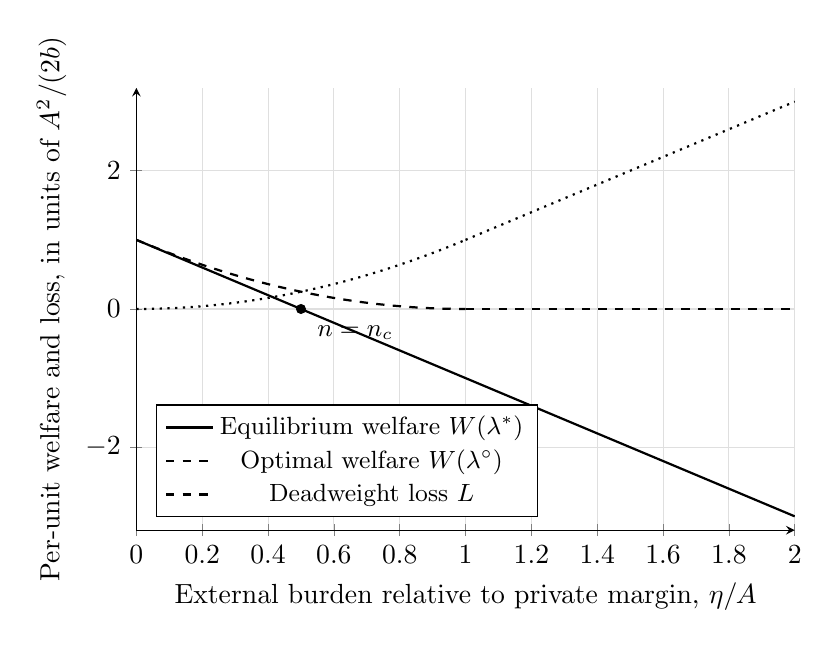
\begin{tikzpicture}
\begin{axis}[
  width=0.82\textwidth, height=7.2cm,
  xlabel={External burden relative to private margin, $\eta/A$},
  ylabel={Per-unit welfare and loss, in units of $A^2/(2b)$},
  xmin=0, xmax=2, ymin=-3.2, ymax=3.2,
  axis lines=left, grid=major, grid style={gray!25},
  legend pos=south west, legend style={font=\small},
  samples=60
]
\addplot[thick, domain=0:2] {1-2*x};
\addlegendentry{Equilibrium welfare $W(\lambda^*)$}
\addplot[thick, dashed, domain=0:1] {(1-x)^2};
\addplot[thick, dashed, domain=1:2] {0};
\addlegendentry{Optimal welfare $W(\lambda^\circ)$}
\addplot[thick, dotted, domain=0:1] {x^2};
\addplot[thick, dotted, domain=1:2] {2*x-1};
\addlegendentry{Deadweight loss $L$}
\addplot[only marks, mark=*, mark size=1.6pt] coordinates {(0.5,0)};
\node[anchor=north west, font=\small] at (axis cs:0.52,-0.1) {$n=n_c$};
\end{axis}
\end{tikzpicture}
\caption{Normalized curves from Theorem~\ref{thm:wedge}. The horizontal axis is $\eta/A=(n-1)h/A$, so that it increases with the size of the audible set. Equilibrium welfare crosses zero at $\eta/A=1/2$, the critical size $n_c$ of Theorem~\ref{thm:divergence}. The figure is a plot of formulas and represents no empirical quantity.}\label{fig:welfare}
\end{figure}

The equilibrium is perpetual in the sense that nothing in it tends to end: every owner's dominant strategy is the same irrespective of what the others do, the external bundle is outside every owner's ledger, and the receipts that measure the activity rise with the very congestion that makes it harmful. A reader who looks at output sees growth, and a resident who looks out of the window sees a city converting the remaining useful life of its buildings into receipts.

\begin{nonsupport}\label{ns:equilibrium}
Theorem~\ref{thm:wedge} and Theorem~\ref{thm:divergence} do not support H and cannot prove it. They are algebraic consequences of a quadratic benefit, a constant harm per unit renovation rate, and an assumption that owners bear no external cost. If owners are liable, if renovation is contracted with the neighbors' consent, or if harm saturates as in Section~\ref{sec:collapse}, the conclusions change or vanish. Moreover, the critical size $n_c=1+A/(2h)$ lies in the linear-harm regime only if $n_c\epsilon$ is small, and the paper does not show that it is. The Perpetual Reconstruction Equilibrium is a defined object whose existence in any actual city is not established.
\end{nonsupport}

\section{The Shangri-La Limit}\label{sec:shangri}

The results so far describe how silence is lost as the audible set grows. The opposite end of the parameter range is the empty audible set, and literature has already supplied it. In Hilton's \emph{Lost Horizon}~\cite{hilton}, a party of evacuees is carried by a hijacked aircraft over the mountains and delivered to Shangri-La, a lamasery in the Kuen-Lun range, equipped with modern comforts and a large library and supplied by a fertile valley. Its residents age slowly, its founder, the High Lama Perrault, is described as roughly two and a half centuries old, and those who leave are said to age rapidly. The protagonist, Conway, is named successor to the High Lama and nevertheless departs with a younger companion, after which his fate is left open. In the vocabulary of this paper, the valley is a place with $n=0$.

\begin{definition}[Shangri-La Condition]
A location satisfies the \emph{Shangri-La Condition} if its audible set is empty, so that $n=0$ and the spatial density $\nu$ of active sources within audible range is zero.
\end{definition}

Every earlier result becomes trivial under the condition, and the triviality is informative about what the results measure. Theorem~\ref{thm:commons} gives silence probability $(1-\epsilon)^0=1$ for every duty cycle. Theorem~\ref{thm:olbers} gives $\E[J]=0$. In Proposition~\ref{prop:chain}, a valley whose components do not become obsolete has $\omega=0$, so that $\lambda=\mu$ and $p_G=0$: the lamasery is maintained and never renovated, and its replacement rate is the rate of its decay. The valley is the point at which the ledger and the physical state of the building coincide.

The literary question is why anyone leaves. The model offers a formal answer based on the bounded harm of Section~\ref{sec:collapse}. Let a resident who lives in a place with audible set $n$ receive an agglomeration benefit $B(n)$, with $B(0)=0$, $B$ nondecreasing, representing access to work, companions, markets and the other goods of density, and suffer a harm $vD_n$ where $D_n = 1-(1-\epsilon)^n$ is the disturbed fraction of time and $v>0$ is the value placed on its elimination. The resident's utility is $U(n)=B(n)-vD_n$, and the valley offers $U(0)=0$.

\begin{proposition}[Conway's Dilemma]\label{prop:conway}
If $B$ is unbounded, then for every duty cycle $\epsilon\in(0,1)$ and every harm value $v>0$ there is a size $\bar n$ such that $U(n)>U(0)$ for all $n\ge\bar n$. In particular, if $B(n)=\beta\ln(1+n)$ with $\beta>0$, then one may take $\bar n = \lceil e^{v/\beta}-1\rceil$ and the threshold does not depend on $\epsilon$.
\end{proposition}

\begin{proof}
Since $0\le D_n<1$, one has $U(n)\ge B(n)-v$. Unboundedness of $B$ gives $\bar n$ with $B(n)>v$ for all $n\ge\bar n$, so that $U(n)>0=U(0)$. For the logarithmic benefit, $\beta\ln(1+n)>v$ if and only if $n>e^{v/\beta}-1$.
\end{proof}

The proposition says that a resident of a sufficiently large city who declines the silent valley is not irrational. Harm saturates at $v$ while the benefit of density does not, so that past a threshold which does not depend on how noisy each unit is, the city dominates the valley in the resident's own accounts. Conway's own motive for leaving, attachment to a younger companion, is a term of $B$ in this reading. The result also complements Proposition~\ref{prop:collapse}: the same saturation that prices the marginal jackhammer at zero makes the noise tolerable, in the sense of utility, to those who can no longer imagine it absent.

A further formal question concerns the name. The novel gave English the word for an idyllic and isolated paradise~\cite{wikishangrila}, and a county-level town in Yunnan was renamed Shangri-La in 2001 in order to promote tourism~\cite{wikishangrila}. A silent place that advertises its silence has an audience, and the audience is made of units. Let the baseline audible set be $n_0\ge0$, and suppose that the number of added units is proportional to the current silence probability, with attraction parameter $m>0$, each added unit (a guesthouse, a restaurant, a road) having the duty cycle $\epsilon$ of Section~\ref{sec:commons}. Treating $n$ as a real number for the purpose of the fixed point, the self-consistent audible set $n^*$ satisfies
\begin{equation}\label{eq:fixedpoint}
n^* = n_0 + m\,(1-\epsilon)^{n^*}.
\end{equation}

\begin{proposition}[Shangri-La Paradox]\label{prop:paradox}
Equation \eqref{eq:fixedpoint} has a unique solution $n^*\ge n_0$. The solution $n^*$ is strictly increasing in $m$, the equilibrium silence probability $s^*=(1-\epsilon)^{n^*}$ is strictly decreasing in $m$, and $n^*\to\infty$ and $s^*\to0$ as $m\to\infty$. At the solution, $s^*=(n^*-n_0)/m$.
\end{proposition}

\begin{proof}
Let $\Phi(n,m)=n-n_0-m(1-\epsilon)^n$. Then $\Phi(n_0,m)=-m(1-\epsilon)^{n_0}<0$, $\Phi\to\infty$ as $n\to\infty$, and $\partial_n\Phi = 1+m|\ln(1-\epsilon)|(1-\epsilon)^n>0$, so there is a unique root. Since $\partial_m\Phi=-(1-\epsilon)^n<0$, the implicit function theorem gives $dn^*/dm=(1-\epsilon)^{n^*}/\partial_n\Phi>0$, and $ds^*/dm=s^*\ln(1-\epsilon)\,dn^*/dm<0$. If $n^*$ were bounded above by $N$ as $m\to\infty$, then $n^*-n_0=m(1-\epsilon)^{n^*}\ge m(1-\epsilon)^N\to\infty$, a contradiction, so $n^*\to\infty$ and hence $s^*=(1-\epsilon)^{n^*}\to0$. The last identity is a rearrangement of \eqref{eq:fixedpoint}.
\end{proof}

Advertising a silent place is accordingly a technology for ending its silence. The more strongly the place is promoted, the larger the audible set at equilibrium and the lower its silence, and in the limit the valley converges to the city. The valley can retain the Shangri-La Condition only if the attraction parameter is zero, which is to say only if no one knows its name.

\begin{nonsupport}\label{ns:shangri}
Proposition~\ref{prop:conway} and Proposition~\ref{prop:paradox} do not support H, and neither describes any actual place. The paper has no data on noise in the town renamed Shangri-La, makes no claim that it exhibits the paradox, and cites the renaming only for a formal analogy. The novel is a work of fiction, its valley is not offered as a policy, and the paper does not establish that any resident of any city would, or should, move to a place with an empty audible set. The assumption that attraction is proportional to silence is a modeling convenience with no empirical support offered here.
\end{nonsupport}

\section{Discussion and Limits}\label{sec:discussion}

The models above are deliberately stylized, and their principal use is to isolate which parameters would have to be measured for H to be tested. These are the gratuitous fraction $p_G$ of Proposition~\ref{prop:chain}, the duty cycle $\epsilon$ and audible set size $n$ of Theorem~\ref{thm:commons}, the mean free path $\ell$ of Theorem~\ref{thm:olbers}, and the harm per unit rate $h$ of Theorem~\ref{thm:wedge}. None of the five has been measured here. The environmental noise guidelines issued for the European region concentrate on transport, wind turbine and leisure sources~\cite{who}, and the acoustic ecology literature offers a vocabulary for the soundscape of a place but no inventory of its renovation duty cycle~\cite{schafer}. Statutory regimes in Japan and in the People's Republic of China regulate construction noise, including breaker work and, in the Chinese case, interior renovation of occupied residential buildings~\cite{japanlaw,chinalaw}, and the existence of such provisions shows that the problem is recognized and not that it is large.

The best counterexample to H available to the author is structural. A substantial share of new apartments in Chinese cities is sold as bare shells, so that initial fit-out is a standard step in occupying a dwelling and not an optional upgrade. Fit-out of that kind is necessary in the sense of Section~\ref{sec:setting}, and it produces exactly the percussive noise that the complaint genre describes. Likewise, tenant turnover, seismic and fire retrofits, water-damage repairs, the replacement of failed membranes beneath tile, and the removal of hazardous materials all produce demolition noise that is not gratuitous. A city could emit continual jackhammer noise with a gratuitous fraction of zero, and Theorems~\ref{thm:commons} and~\ref{thm:olbers} would apply unchanged. The complaints in the genre are therefore compatible with a world in which no renovation is unnecessary and the sole defect is the aggregate.

Layered building theory is a further source of caution. Brand~\cite{brand} describes buildings as composed of layers that change at different rates, with the interior fit-out changing fastest. A high renovation rate of interior finishes is thus an expected property of occupied buildings and not in itself an anomaly. Baumol's analysis of unbalanced growth~\cite{baumol} adds that labor-intensive trades such as tile setting become relatively more expensive over time, which pushes $c$ upward and shrinks the private margin $A$ in Section~\ref{sec:equilibrium}, against the equilibrium. Depreciation and tax conventions in some regimes can set a ledger life distinct from physical life, which would raise $I_k$ in \eqref{eq:ledger}, but the paper does not assert the magnitude of this effect in any jurisdiction.

The threats to validity are numerous. The duty cycle is treated as stationary and homogeneous. Sources are treated as identical. Sound is treated as an isotropic scalar and not as the mixture of airborne and structure-borne paths that characterizes real buildings. Harm is treated as linear in Section~\ref{sec:equilibrium} and as binary in Section~\ref{sec:collapse}. Owners are treated as a homogeneous population with a common price, and no model of contractors, tenants, lenders or regulators is offered. The video commentary that motivates the paper is not a sample of any population, is selected for complaint, and is produced by speakers who may be unusually sensitive, unusually present in their dwellings, or unusually positioned to compare their circumstances with those of other places.

\begin{nonsupport}\label{ns:discussion}
Nothing in this discussion supports H. The discussion in fact supplies reasons to doubt H, and the paper regards the doubt as better supported than the hypothesis. The fraction of urban demolition noise attributable to gratuitous replacement is a number between zero and one that the paper does not bound away from either end.
\end{nonsupport}

\section{Conclusion}\label{sec:conclusion}

Seven conditional results have been proved. Under ledger-driven replacement the replaced stock is a representative sample of the whole, and with fast obsolescence and readiness the replacement rate is insensitive to decay to first order. Under independence the probability of silence in an audible set of $n$ units is $(1-\epsilon)^n$, and under statutory working hours the only quiet that survives at scale is the quiet that the statute mandates. In a Poisson field the mean acoustic intensity is the product of the density of active sources, their typical power and the mean free path of the structure, with the nearest source controlling the fluctuation. A marginal-harm fee tends to zero as the audience saturates. In a symmetric game in which owners bear no external cost, there is a critical audible set size beyond which measured output rises while welfare is negative. A resident of a sufficiently large city is better off there than in an empty valley whatever the noise per unit, because harm saturates and the benefits of density do not, and a silent place that advertises its silence loses it in proportion to the advertising.

Within the models above, and only within them, one may therefore state the following proposition, in which the word \emph{limiting} carries all of the weight. In the limiting case of metropolitan saturation, a city can be described as an apparatus that converts the remaining useful life of its buildings into contractor revenue, particulate matter and acoustic burden, while its accounts record the conversion as growth, and its inhabitants are invited to regard the process as progress. This proposition is a corollary of the assumptions and not of the world. The paper has not shown that it describes Tokyo, any Chinese city, or any other place, it has not shown that any floor was broken out without cause, and it has not proved the hypothesis that motivated it. The jackhammer, meanwhile, continues.

\begin{thebibliography}{99}

\bibitem{baumol}
Baumol, W. J. Macroeconomics of Unbalanced Growth: The Anatomy of Urban Crisis. \emph{American Economic Review} 57(3), 415--426, 1967.

\bibitem{bastiat}
Bastiat, F. That Which Is Seen and That Which Is Not Seen. Originally published as \emph{Ce qu'on voit et ce qu'on ne voit pas}, 1850.

\bibitem{brand}
Brand, S. \emph{How Buildings Learn: What Happens After They're Built}. New York: Viking, 1994.

\bibitem{campbell}
Campbell, N. R. The Study of Discontinuous Phenomena. \emph{Proceedings of the Cambridge Philosophical Society} 15, 117--136, 1909.

\bibitem{chinalaw}
National People's Congress of the People's Republic of China. Law of the People's Republic of China on the Prevention and Control of Noise Pollution. Adopted 1996, revised 2021.

\bibitem{coase}
Coase, R. H. The Problem of Social Cost. \emph{Journal of Law and Economics} 3, 1--44, 1960.

\bibitem{cover}
Cover, T. M., and Thomas, J. A. \emph{Elements of Information Theory}, 2nd ed. Hoboken: Wiley, 2006.

\bibitem{cox}
Cox, D. R., and Smith, W. L. On the Superposition of Renewal Processes. \emph{Biometrika} 41, 91--99, 1954.

\bibitem{hardin}
Hardin, G. The Tragedy of the Commons. \emph{Science} 162, 1243--1248, 1968.

\bibitem{harrison}
Harrison, E. R. \emph{Darkness at Night: A Riddle of the Universe}. Cambridge, MA: Harvard University Press, 1987.

\bibitem{hilton}
Hilton, J. \emph{Lost Horizon}. London: Macmillan, 1933.

\bibitem{japanlaw}
Government of Japan. Noise Regulation Law. Enacted 1968.

\bibitem{jensen}
Jensen, M. C., and Meckling, W. H. Theory of the Firm: Managerial Behavior, Agency Costs and Ownership Structure. \emph{Journal of Financial Economics} 3, 305--360, 1976.

\bibitem{khinchin}
Khinchin, A. Y. \emph{Mathematical Methods in the Theory of Queueing}. London: Griffin, 1960.

\bibitem{kingman}
Kingman, J. F. C. \emph{Poisson Processes}. Oxford: Oxford University Press, 1993.

\bibitem{olson}
Olson, M. \emph{The Logic of Collective Action: Public Goods and the Theory of Groups}. Cambridge, MA: Harvard University Press, 1965.

\bibitem{ostrom}
Ostrom, E. \emph{Governing the Commons: The Evolution of Institutions for Collective Action}. Cambridge: Cambridge University Press, 1990.

\bibitem{pigou}
Pigou, A. C. \emph{The Economics of Welfare}. London: Macmillan, 1920.

\bibitem{schafer}
Schafer, R. M. \emph{The Soundscape: Our Sonic Environment and the Tuning of the World}. Rochester: Destiny Books, 1977.

\bibitem{schumpeter}
Schumpeter, J. A. \emph{Capitalism, Socialism and Democracy}. New York: Harper and Brothers, 1942.

\bibitem{veblen}
Veblen, T. \emph{The Theory of the Leisure Class}. New York: Macmillan, 1899.

\bibitem{who}
World Health Organization Regional Office for Europe. \emph{Environmental Noise Guidelines for the European Region}. Copenhagen: WHO, 2018.

\bibitem{wikishangrila}
Wikipedia. Shangri-La. Accessed October 2026. \url{https://en.wikipedia.org/wiki/Shangri-La}; and Wikipedia. Lost Horizon. Accessed October 2026. \url{https://en.wikipedia.org/wiki/Lost_Horizon}.

\end{thebibliography}

\end{document}
